% tikzpic.tex
\documentclass[crop,tikz]{standalone}% 'crop' is the default for v1.0, before it was 'preview'

\usetikzlibrary{arrows,decorations.pathmorphing,decorations.pathreplacing,backgrounds,positioning,fit,matrix}
\usetikzlibrary{shapes,calc,patterns,arrows.meta}
\tikzset{
	vert/.style={circle,inner sep=1.5,fill=white,draw,minimum size=.3cm},
	edge/.style={color=black, thick},
	diredge/.style={->,>={Stealth[width=8pt,length=8pt]},color=black, thick},
	timelabel/.style={fill=white,font=\footnotesize, text centered},
	wave/.style={decorate,decoration={coil,aspect=0}},
	dirwave/.style={->, >={Stealth[width=8pt,length=8pt]},decorate,decoration={coil,aspect=0}},
	diredge2/.style={->,>={Stealth[width=8pt,length=8pt]}}
}
\begin{document}
	
	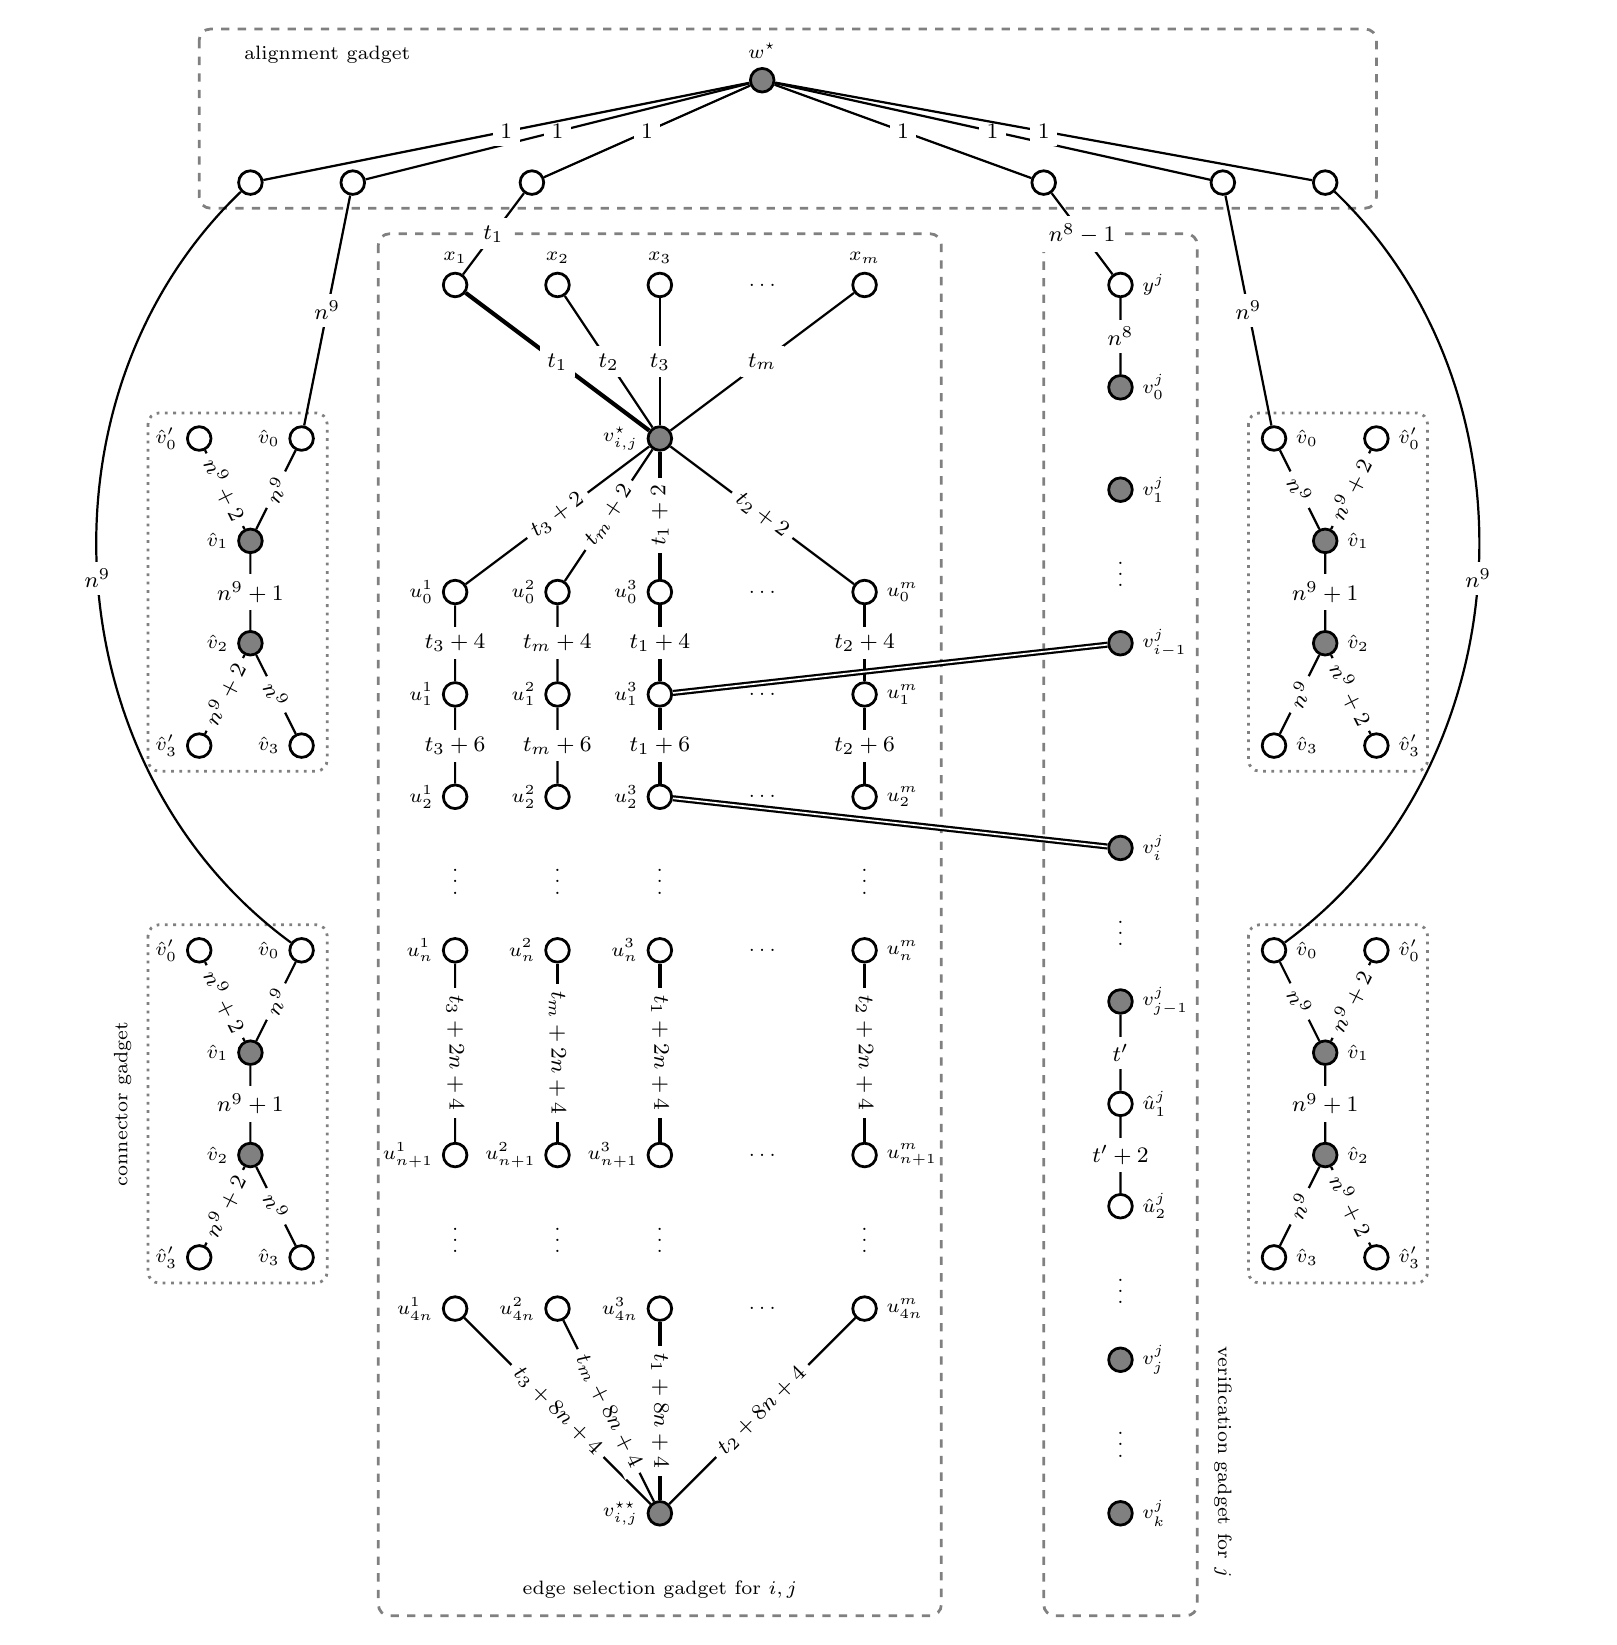
\begin{tikzpicture}[line width=1pt, scale=.65]
		\scriptsize
		\node (A) at (14,0) {};
		
		\draw[rounded corners, dashed, gray] (-13, 5) rectangle (10, 1.5) {};
		\node (A) at (-10.5,4.5) {alignment gadget};
		
		\draw[rounded corners, dotted, gray] (-14, -2.5) rectangle (-10.5, -9.5) {};
		\draw[rounded corners, dotted, gray] (-14, -12.5) rectangle (-10.5, -19.5) {};
		\draw[rounded corners, dotted, gray] (7.5, -2.5) rectangle (11, -9.5) {};
		\draw[rounded corners, dotted, gray] (7.5, -12.5) rectangle (11, -19.5) {};
		\node[rotate=90] (A) at (-14.5,-16) {connector gadget};
		
		\draw[rounded corners, dashed, gray] (-9.5, 1) rectangle (1.5, -26) {};
		\node (A) at (-4,-25.5) {edge selection gadget for $i,j$};
		
		\draw[rounded corners, dashed, gray] (3.5, 1) rectangle (6.5, -26) {};
		\node[rotate=-90] (A) at (7,-23) {verification gadget for $j$};
		
		\node[vert,label=above:$w^\star$, fill=gray] (W) at (-2,4) {};
		\node[vert] (W1) at (-6.5,2) {};
		\node[vert] (W2) at (-10,2) {};
		\node[vert] (W3) at (-12,2) {};
		\node[vert] (W4) at (7,2) {}; 
		\node[vert] (W5) at (3.5,2) {};
		\node[vert] (W6) at (9,2) {}; 
		
		
		\node[vert,label=left:$\hat{v}_0$] (VH11) at (-11,-3) {}; 
		\node[vert,label=left:$\hat{v}_0'$] (VH111) at (-13,-3) {}; 
		\node[vert,label=left:$\hat{v}_1$, fill=gray] (VH12) at (-12,-5) {}; 
		\node[vert,label=left:$\hat{v}_2$, fill=gray] (VH13) at (-12,-7) {}; 
		\node[vert,label=left:$\hat{v}_3$] (VH14) at (-11,-9) {};  
		\node[vert,label=left:$\hat{v}_3'$] (VH144) at (-13,-9) {}; 
		
		\node[vert,label=left:$\hat{v}_0$] (VH21) at (-11,-13) {};
		\node[vert,label=left:$\hat{v}_0'$] (VH211) at (-13,-13) {}; 
		\node[vert,label=left:$\hat{v}_1$, fill=gray] (VH22) at (-12,-15) {}; 
		\node[vert,label=left:$\hat{v}_2$, fill=gray] (VH23) at (-12,-17) {};
		\node[vert,label=left:$\hat{v}_3$] (VH24) at (-11,-19) {};
		\node[vert,label=left:$\hat{v}_3'$] (VH244) at (-13,-19) {}; 
		
		\node[vert,label=right:$\hat{v}_0$] (VH31) at (8,-3) {}; 
		\node[vert,label=right:$\hat{v}_0'$] (VH311) at (10,-3) {}; 
		\node[vert,label=right:$\hat{v}_1$, fill=gray] (VH32) at (9,-5) {}; 
		\node[vert,label=right:$\hat{v}_2$, fill=gray] (VH33) at (9,-7) {}; 
		\node[vert,label=right:$\hat{v}_3$] (VH34) at (8,-9) {};  
		\node[vert,label=right:$\hat{v}_3'$] (VH344) at (10,-9) {}; 
		
		\node[vert,label=right:$\hat{v}_0$] (VH41) at (8,-13) {}; 
		\node[vert,label=right:$\hat{v}_0'$] (VH411) at (10,-13) {}; 
		\node[vert,label=right:$\hat{v}_1$, fill=gray] (VH42) at (9,-15) {}; 
		\node[vert,label=right:$\hat{v}_2$, fill=gray] (VH43) at (9,-17) {}; 
		\node[vert,label=right:$\hat{v}_3$] (VH44) at (8,-19) {};  
		\node[vert,label=right:$\hat{v}_3'$] (VH444) at (10,-19) {}; 
		
		\node[vert,label=above:$x_1$] (X1) at (-8,0) {}; 
		\node[vert,label=above:$x_2$] (X2) at (-6,0) {}; 
		\node[vert,label=above:$x_3$] (X3) at (-4,0) {}; 
		\node (A) at (-2,0) {$\ldots$};
		\node[vert,label=above:$x_m$] (XM) at (0,0) {}; 
		
		\node[vert,label=left:$v_{i,j}^\star$, fill=gray] (VS) at (-4,-3) {}; 
		
		\node[vert,label=left:$u^1_0$] (Y1) at (-8,-6) {}; 
		\node[vert,label=left:$u^2_0$] (Y2) at (-6,-6) {}; 
		\node[vert,label=left:$u^3_0$] (Y3) at (-4,-6) {}; 
		\node (A) at (-2,-6) {$\ldots$};
		\node[vert,label=right:$u^m_0$] (YM) at (0,-6) {}; 
		
		\node[vert,label=left:$u^1_1$] (U11) at (-8,-8) {}; 
		\node[vert,label=left:$u^2_1$] (U12) at (-6,-8) {}; 
		\node[vert,label=left:$u^3_1$] (U13) at (-4,-8) {}; 
		\node (A) at (-2,-8) {$\ldots$};
		\node[vert,label=right:$u^m_1$] (U1M) at (0,-8) {};
		
		\node[vert,label=left:$u^1_2$] (U21) at (-8,-10) {}; 
		\node[vert,label=left:$u^2_2$] (U22) at (-6,-10) {}; 
		\node[vert,label=left:$u^3_2$] (U23) at (-4,-10) {}; 
		\node (A) at (-2,-10) {$\ldots$};
		\node[vert,label=right:$u^m_2$] (U2M) at (0,-10) {};
		
		\node (A) at (-8,-11.5) {$\vdots$}; 
		\node (A) at (-6,-11.5) {$\vdots$}; 
		\node (A) at (-4,-11.5) {$\vdots$}; 
		\node (A) at (0,-11.5) {$\vdots$};
		
		\node[vert,label=left:$u^1_n$] (UN1) at (-8,-13) {}; 
		\node[vert,label=left:$u^2_n$] (UN2) at (-6,-13) {}; 
		\node[vert,label=left:$u^3_n$] (UN3) at (-4,-13) {}; 
		\node (A) at (-2,-13) {$\ldots$};
		\node[vert,label=right:$u^m_n$] (UNM) at (0,-13) {};
		
		\node[vert,label=left:$u_{n+1}^1$] (UN11) at (-8,-17) {}; 
		\node[vert,label=left:$u_{n+1}^2$] (UN12) at (-6,-17) {}; 
		\node[vert,label=left:$u_{n+1}^3$] (UN13) at (-4,-17) {}; 
		\node (A) at (-2,-17) {$\ldots$};
		\node[vert,label=right:$u_{n+1}^m$] (UN1M) at (0,-17) {};
		
		\node (A) at (-8,-18.5) {$\vdots$}; 
		\node (A) at (-6,-18.5) {$\vdots$}; 
		\node (A) at (-4,-18.5) {$\vdots$}; 
		\node (A) at (0,-18.5) {$\vdots$};
		
		\node[vert,label=left:$u_{4n}^1$] (U2N1) at (-8,-20) {}; 
		\node[vert,label=left:$u_{4n}^2$] (U2N2) at (-6,-20) {}; 
		\node[vert,label=left:$u_{4n}^3$] (U2N3) at (-4,-20) {}; 
		\node (A) at (-2,-20) {$\ldots$};
		\node[vert,label=right:$u_{4n}^m$] (U2NM) at (0,-20) {};
		
		\node[vert,label=left:$v_{i,j}^{\star\star}$, fill=gray] (VSS) at (-4,-24) {};
		
		
		\node[vert,label=right:$y^j$] (YI) at (5,0) {};
		\node[vert,label=right:$v_0^j$, fill=gray] (VI0) at (5,-2) {};
		\node[vert,label=right:$v_1^j$, fill=gray] (VI1) at (5,-4) {};
		\node (A) at (5,-5.5) {$\vdots$};
		\node[vert,label=right:$v_{i-1}^j$, fill=gray] (VIJ1) at (5,-7) {};
		\node[vert,label=right:$v_{i}^j$, fill=gray] (VIJ) at (5,-11) {};
		\node (A) at (5,-12.5) {$\vdots$};
		\node[vert,label=right:$v_{j-1}^j$, fill=gray] (VII1) at (5,-14) {};
		\node[vert,label=right:$\hat{u}_{1}^j$] (UI1) at (5,-16) {};
		\node[vert,label=right:$\hat{u}_{2}^j$] (UI2) at (5,-18) {};
		\node (A) at (5,-19.5) {$\vdots$};
		\node[vert,label=right:$v_{j}^j$, fill=gray] (UIN3) at (5,-21) {};
		\node (A) at (5,-22.5) {$\vdots$};
		\node[vert,label=right:$v_{k}^j$, fill=gray] (VIK) at (5,-24) {};
		
		\draw[edge, line width=1.5pt] (X1) --node[timelabel] {$t_1$} (VS);
		\draw[edge] (X2) --node[timelabel] {$t_2$} (VS);
		\draw[edge] (X3) --node[timelabel] {$t_3$} (VS);
		\draw[edge] (XM) --node[timelabel] {$t_m$} (VS);
		
		\draw[edge] (Y1) --node[timelabel,sloped] {$t_3+2$} (VS);
		\draw[edge] (Y2) --node[timelabel,sloped] {$t_m+2$} (VS);
		\draw[edge, line width=1.5pt] (Y3) --node[timelabel,sloped] {$t_1+2$} (VS);
		\draw[edge] (YM) --node[timelabel,sloped] {$t_2+2$} (VS);
		
		\draw[edge] (Y1) --node[timelabel] {$t_3+4$} (U11);
		\draw[edge] (Y2) --node[timelabel] {$t_m+4$} (U12);
		\draw[edge, line width=1.5pt] (Y3) --node[timelabel] {$t_1+4$} (U13);
		\draw[edge] (YM) --node[timelabel] {$t_2+4$} (U1M);
		
		\draw[edge] (U21) --node[timelabel] {$t_3+6$} (U11);
		\draw[edge] (U22) --node[timelabel] {$t_m+6$} (U12);
		\draw[edge, line width=1.5pt] (U23) --node[timelabel] {$t_1+6$} (U13);
		\draw[edge] (U2M) --node[timelabel] {$t_2+6$} (U1M);
		
		\draw[edge] (UN1) --node[timelabel,sloped] {$t_3+2n+4$} (UN11);
		\draw[edge] (UN2) --node[timelabel,sloped] {$t_m+2n+4$} (UN12);
		\draw[edge, line width=1.5pt] (UN3) --node[timelabel,sloped] {$t_1+2n+4$} (UN13);
		\draw[edge] (UNM) --node[timelabel,sloped] {$t_2+2n+4$} (UN1M);
		
		\draw[edge] (U2N1) --node[timelabel,sloped] {$t_3+8n+4$} (VSS);
		\draw[edge] (U2N2) --node[timelabel,sloped] {$t_m+8n+4$} (VSS);
		\draw[edge, line width=1.5pt] (U2N3) --node[timelabel,sloped] {$t_1+8n+4$} (VSS);
		\draw[edge] (U2NM) --node[timelabel,sloped] {$t_2+8n+4$} (VSS);
		
		\draw[edge] (VH11) --node[timelabel,sloped] {$n^9$} (VH12);
		\draw[edge] (VH12) --node[timelabel,sloped] {$n^9+2$} (VH111);
		\draw[edge] (VH12) --node[timelabel] {$n^9+1$} (VH13);
		\draw[edge] (VH13) --node[timelabel,sloped] {$n^9$} (VH14);
		\draw[edge] (VH13) --node[timelabel,sloped] {$n^9+2$} (VH144);
		
		\draw[edge] (VH21) --node[timelabel,sloped] {$n^9$} (VH22);
		\draw[edge] (VH22) --node[timelabel,sloped] {$n^9+2$} (VH211);
		\draw[edge] (VH22) --node[timelabel] {$n^9+1$} (VH23);
		\draw[edge] (VH23) --node[timelabel,sloped] {$n^9$} (VH24);
		\draw[edge] (VH23) --node[timelabel,sloped] {$n^9+2$} (VH244);
		
		\draw[edge] (VH31) --node[timelabel,sloped] {$n^9$} (VH32);
		\draw[edge] (VH32) --node[timelabel,sloped] {$n^9+2$} (VH311);
		\draw[edge] (VH32) --node[timelabel] {$n^9+1$} (VH33);
		\draw[edge] (VH33) --node[timelabel,sloped] {$n^9$} (VH34);	
		\draw[edge] (VH33) --node[timelabel,sloped] {$n^9+2$} (VH344);
		
		\draw[edge] (VH41) --node[timelabel,sloped] {$n^9$} (VH42);
		\draw[edge] (VH42) --node[timelabel,sloped] {$n^9+2$} (VH411);
		\draw[edge] (VH42) --node[timelabel] {$n^9+1$} (VH43);
		\draw[edge] (VH43) --node[timelabel,sloped] {$n^9$} (VH44);	
		\draw[edge] (VH43) --node[timelabel,sloped] {$n^9+2$} (VH444);
		
		%\draw[edge] (VIJ1) --node[timelabel, near start] {$t_1+4$} (U13);
		%\draw[edge] (VIJ) --node[timelabel, near start] {$t_1+8$} (U23);
		
		\draw[edge,double] (VIJ1) --node {} (U13);
		\draw[edge,double] (VIJ) --node {} (U23);
		
		
		\draw[edge] (W) --node[timelabel] {$1$} (W1);
		\draw[edge] (W) --node[timelabel] {$1$} (W2);
		\draw[edge] (W) --node[timelabel] {$1$} (W3);
		\draw[edge] (W) --node[timelabel] {$1$} (W4);
		\draw[edge] (W) --node[timelabel] {$1$} (W5);
		\draw[edge] (W) --node[timelabel] {$1$} (W6);
		
		\draw[edge] (X1) --node[timelabel] {$t_1$} (W1);
		\draw[edge] (VH11) --node[timelabel] {$n^9$} (W2);
		\draw[edge] (VH21) edge[bend left=50] node[timelabel] {$n^9$} (W3);
		\draw[edge] (VH31) --node[timelabel] {$n^9$} (W4);
		\draw[edge] (YI) --node[timelabel] {$n^8-1$} (W5);
		\draw[edge] (VH41) edge[bend right=50] node[timelabel] {$n^9$} (W6);
		
		\draw[edge] (YI) --node[timelabel] {$n^8$} (VI0);
		
		\draw[edge] (VII1) --node[timelabel] {$t'$} (UI1);
		\draw[edge] (UI1) --node[timelabel] {$t'+2$} (UI2);
	\end{tikzpicture}
	
\end{document}